\documentclass[11pt]{article}
\usepackage{geometry}                % See geometry.pdf to learn the layout options. There are lots.
\geometry{letterpaper}                   % ... or a4paper or a5paper or ... 
%\geometry{landscape}                % Activate for for rotated page geometry
%\usepackage[parfill]{parskip}    % Activate to begin paragraphs with an empty line rather than an indent
\usepackage{graphicx}
\usepackage{amssymb,amsmath}
\usepackage{epstopdf}
\usepackage{pgf}
\usepackage{pgfpages}
\usepackage{tikz}
\usetikzlibrary{arrows,backgrounds}
\usepgflibrary{shapes}
\DeclareGraphicsRule{.tif}{png}{.png}{`convert #1 `dirname #1`/`basename #1 .tif`.png}
\pagestyle{empty}


\begin{document}

  \begin{center}
   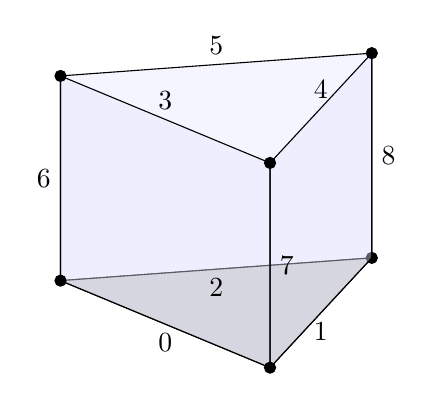
\begin{tikzpicture}[join=round] % Wedge edge numbering
       \filldraw[fill=blue!10,fill opacity=0.4](-2.205,2.872)--(-2.205,.272)--(1.748,.561)--(1.748,3.161)--cycle;
       \filldraw[fill=black!20](1.748,.561)--(-2.205,.272)--(.456,-.833)--cycle;
        \filldraw(1.748,.561) circle (2pt);
       \filldraw[fill=blue!10,fill opacity=0.4](1.748,3.161)--(1.748,.561)--(.456,-.833)--(.456,1.767)--cycle;
       \filldraw[fill=blue!10,fill opacity=0.4](.456,1.767)--(.456,-.833)--(-2.205,.272)--(-2.205,2.872)--cycle;
        \filldraw(-2.205,.272) circle (2pt);
        \filldraw(1.748,3.161) circle (2pt);
        \filldraw(-2.205,2.872) circle (2pt);
        \filldraw(.456,-.833) circle (2pt);
        \filldraw(.456,1.767) circle (2pt);
       \fill[black]
                (-.874,-.281) node [below] {0}
                (1.102,-.136) node [below] {1}
                (-.228,.417) node [below] {2}
                (-.874,2.319) node [above] {3}
                (1.102,2.464) node [above] {4}
                (-.228,3.017) node [above] {5}
                (-2.205,1.572) node [left] {6}
                (.456,.467) node [right] {7}
                (1.748,1.861) node [right] {8};
    \end{tikzpicture}
 \end{center}

\end{document}  
